\documentclass{article}
\usepackage[utf8]{inputenc}

% Page setup
\usepackage[a4paper,landscape,margin=2cm]{geometry}
\usepackage{amsmath}

% Typography
\usepackage[scaled]{helvet}
\let\familydefault\sfdefault

\usepackage[usenames,svgnames]{xcolor}
\usepackage{tikz,pgfplots}
\usetikzlibrary{positioning,arrows,intersections}

\definecolor{colorconfig}     {RGB}{199,212,104}
\definecolor{colorapp}        {RGB}{79 ,142,209}
\definecolor{colorextcomp}    {RGB}{143,232,186}
\definecolor{colorjson}       {RGB}{49 ,167,126}
\definecolor{colortext}       {RGB}{29 ,29 ,27 }
\definecolor{colorinstance}   {RGB}{119 ,182,249}
\definecolor{colorextinstance}{RGB}{163,255,206}
\definecolor{colorcompjs}     {RGB}{255,163,56}

\begin{document}
\pagestyle{empty}
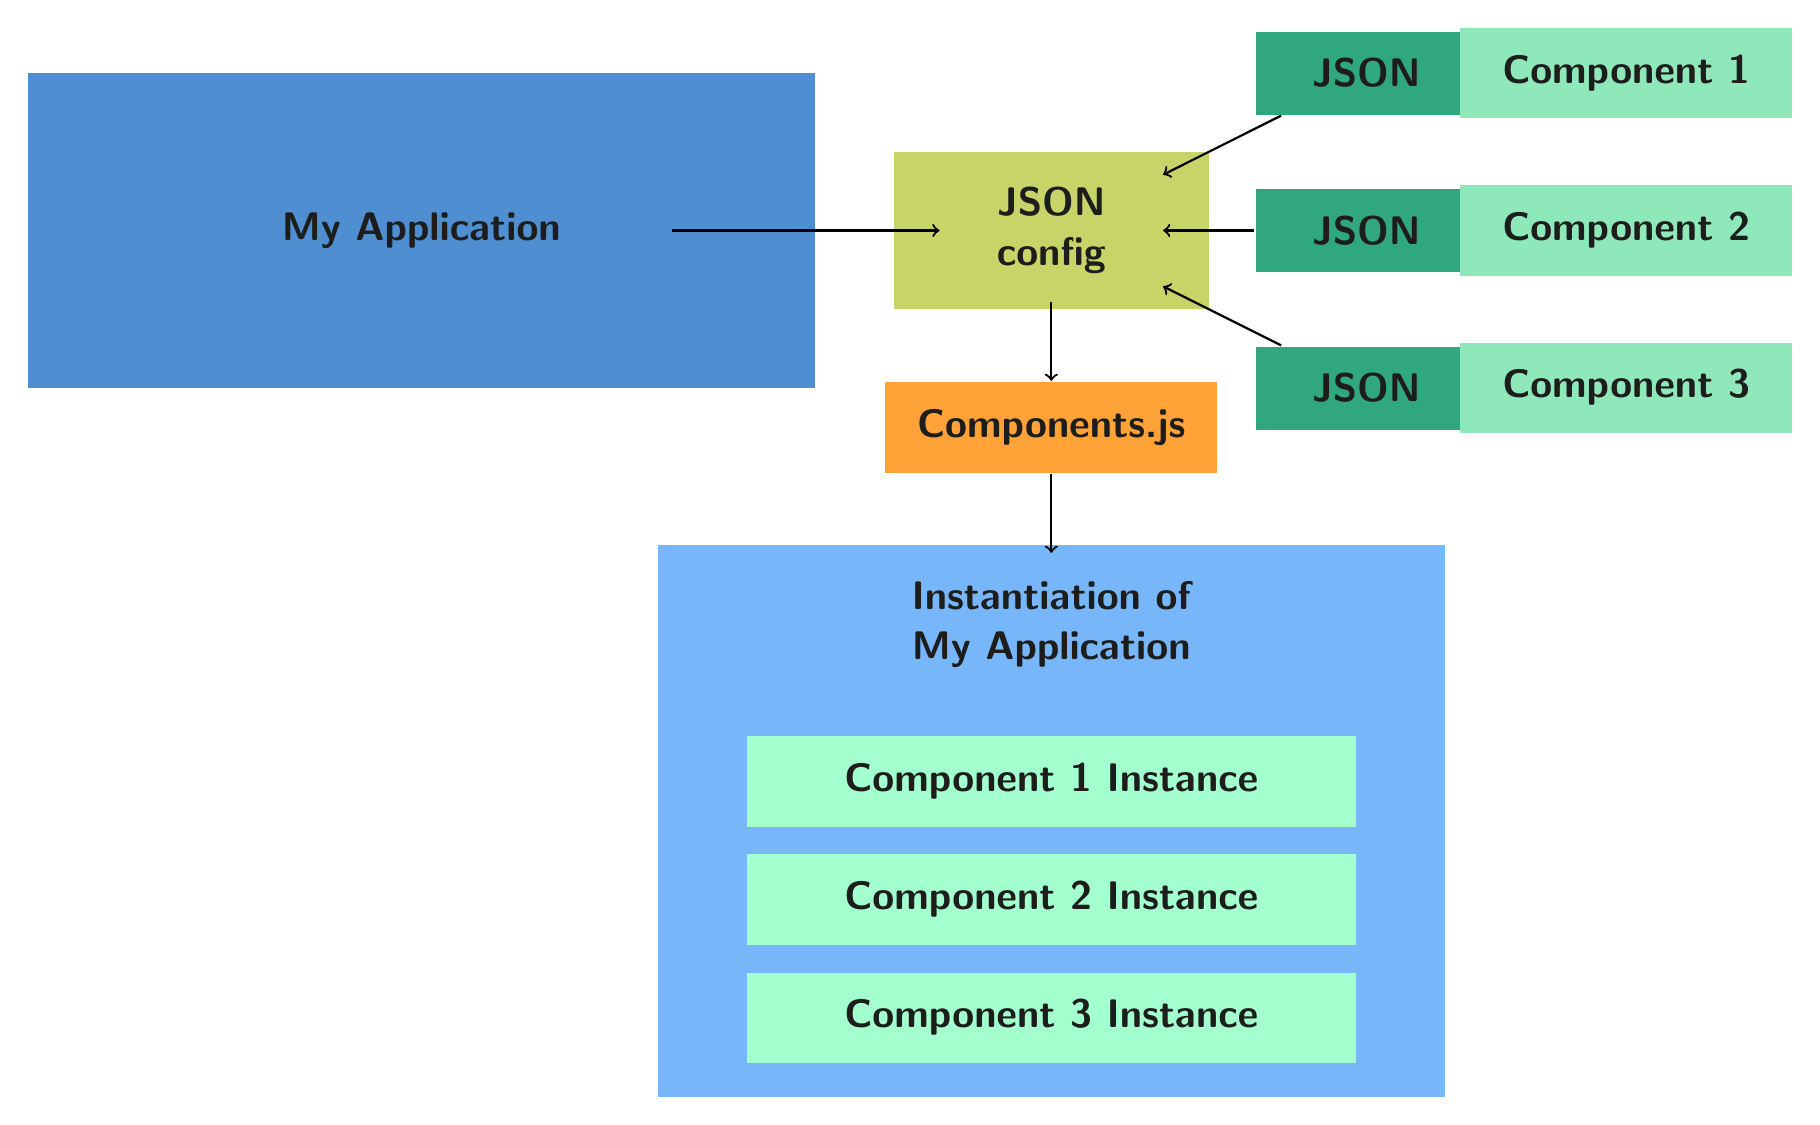
\begin{tikzpicture}[
    node distance = 2em, auto,
    font={\Large\itshape},
    base/.style={text=colortext,font={\Large\bfseries},inner sep=10pt,align=center,rectangle,thick},
    txt/.style={text=colortext,font={\Large\bfseries},align=center},
    relation/.style={text width=13em},
]

    \fill [colorapp] (0,4) rectangle (10,8);
    \node[base,fill=colorapp,text width=16em] at (5,6) (app) {My Application};

    \node[base,fill=colorjson,text width=6em] at (17,8) (comp1config) {JSON};
    \node[base,fill=colorextcomp,text width=10em] at (20.3,8) (comp1) {Component 1};
    \node[base,fill=colorjson,text width=6em] at (17,6) (comp2config) {JSON};
    \node[base,fill=colorextcomp,text width=10em] at (20.3,6) (comp2) {Component 2};
    \node[base,fill=colorjson,text width=6em] at (17,4) (comp3config) {JSON};
    \node[base,fill=colorextcomp,text width=10em] at (20.3,4) (comp3) {Component 3};

    \fill [colorconfig] (11,5) rectangle (15,7);
    \node[base,fill=colorconfig,text width=6em] at (13,6) (config) {JSON\\config};
    
    \node[base,fill=colorcompjs,text width=10em] at (13,3.5) (componentsjs) {Components.js};

    \fill [colorinstance] (8,2) rectangle (18,-5);
    \node[base,fill=colorinstance,text width=16em] at (13,1) (instance) {Instantiation of\\My Application};
    \node[base,fill=colorextinstance,text width=20em] at (13,-1) (inst1) {Component 1 Instance};
    \node[base,fill=colorextinstance,text width=20em] at (13,-2.5) (inst2) {Component 2 Instance};
    \node[base,fill=colorextinstance,text width=20em] at (13,-4) (inst3) {Component 3 Instance};
    
    \draw[->,thick](app) to (config);
    \draw[->,thick](comp1config) to (config);
    \draw[->,thick](comp2config) to (config);
    \draw[->,thick](comp3config) to (config);
    \draw[->,thick](config) to (componentsjs);
    \draw[->,thick](componentsjs) to (instance);

\end{tikzpicture}
\end{document}
